\chapter{Introduction}

\section{Overview of Generative AI}

Generative Artificial Intelligence (GenAI) refers to models that produce new content, such as text, images or
structured data, instead of only assigning a label to an input. Most of the current systems are built on the
Transformer architecture~\cite{vaswani2017attention}. Large Language Models (LLMs) trained on very large text
collections were shown to perform many tasks from a handful of examples in the prompt~\cite{brown2020gpt3}, and
multimodal models such as Gemini accept text, images and other media in one request~\cite{gemini2023,gemini25}.
For an application developer, three capabilities of these models matter most.

\begin{itemize}
\item \textbf{Understanding free-form language and images.} A farmer can ask ``Was the soil drier than yesterday?'' in
      ordinary words, or send a photograph of a leaf, without choosing from a menu.
\item \textbf{Structured output.} A model can be instructed to return JSON that follows a schema. This lets
      deterministic program code, and not the model, decide what happens next.
\item \textbf{Tool use and retrieval.} A model can be given retrieved documents or web search results and asked to
      answer from them. This approach is called Retrieval-Augmented Generation (RAG)~\cite{lewis2020rag,gao2023ragsurvey},
      and a loop in which the model decides what to look up next is the basis of ``agentic''
      systems~\cite{yao2023react,wang2024agents}.
\end{itemize}

The same models also have well-known weaknesses. They can state false information fluently, a behaviour known as
hallucination~\cite{ji2023hallucination}, and their own statements of confidence are not reliable
probabilities~\cite{kadavath2022know,xiong2024uncertainty}. A responsible application therefore has to
decide which parts of an answer may come from a model (wording, explanation) and which parts must come from
verifiable code (numbers, dates, citations). This division is the central design principle of the project described
in this report.

\section{Project Background}

Crop losses often begin as small changes that are only noticed late: a few spotted leaves, a humid spell that favours
fungal disease, or soil that has been drying for days. Two kinds of tools address this today. Mobile applications for
plant disease identification, such as Plantix~\cite{plantix}, are \emph{reactive}: they help only after the farmer has
noticed a problem and photographed it. Sensor kits log temperature, humidity or soil moisture, but their output is a
table or a chart that the farmer has to interpret.

\textbf{GAIA} (the project name) combines the two ideas around a small, low-cost \emph{rover}. The rover carries an
ESP32-CAM, an Arduino Nano, a DHT11 temperature and humidity sensor, MQ-5 and MQ-6 gas sensors and a soil-moisture
probe on a servo-controlled arm. It streams live video to a Flutter mobile application and records field
measurements. The rover is deliberately kept as a thin data-acquisition layer. The substance of the project lies in
two independent Generative AI pipelines that run on a Python backend (Figure~\ref{fig:overview}):

\begin{itemize}
\item \textbf{Pipeline A, the conversational assistant.} In ``Query my farm'' mode it answers questions from the
      farmer's own sensor log, earlier diagnoses and notes. In ``Open-ended'' mode it answers general questions with
      web search.
\item \textbf{Pipeline B, crop diagnosis.} A single vision-language model (VLM) call analyses a photograph and one
      research agent looks up care or treatment information on the web.
\end{itemize}

The two pipelines share one knowledge store (PostgreSQL with the pgvector extension) but have no control-flow
dependency on each other (Figure~\ref{fig:pipelines}).

\begin{figure}[H]
\centering
\scaledtikz{\begin{tikzpicture}
\node[gbox,text width=24mm] (rover) at (0,0) {\textbf{Rover}\\sensors and\\camera};
\node[box,text width=24mm] (ing) at (3.9,0) {\textbf{Ingestion}\\validate, window,\\text chunks};
\node[db,text width=18mm] (kb) at (7.8,0) {\textbf{Knowledge}\\\textbf{store}};
\node[gbox,text width=24mm] (pa) at (11.7,0) {\textbf{Pipeline A}\\sensor-grounded\\RAG chat};
\node[dbox,text width=24mm] (app) at (15.6,0) {\textbf{Flutter app}\\chat, diagnose,\\rover, live view};
\node[box,text width=24mm] (cam) at (0,-3.6) {\textbf{Crop photo}\\rover or phone\\camera};
\node[gbox,text width=36mm] (pb) at (7.8,-3.6) {\textbf{Pipeline B}\\VLM diagnosis +\\one web research agent};
\draw[arr] (rover) -- node[lbl,above]{Wi-Fi} (ing);
\draw[arr] (ing) -- (kb);
\draw[arr] (kb) -- node[lbl,above]{read} (pa);
\draw[arr] (pa) -- node[lbl,above]{SSE} (app);
\draw[arr] (cam) -- (pb);
\draw[arr] (pb) -- node[lbl,right]{one-way write} (kb);
\draw[arr] (pb.east) -| node[lbl,pos=0.2,above]{result and sources} (app.south);
\end{tikzpicture}}

\caption{System overview: the rover feeds ingestion, Pipeline B writes one way into the shared knowledge store, and
Pipeline A reads from it.}
\label{fig:overview}
\end{figure}

\begin{figure}[H]
\centering
\scaledtikz{\begin{tikzpicture}
\node[zlbl] at (4.6,0.9) {no control-flow dependency between the two pipelines};
\node[zlbl] (ta) at (0,0.2) {PIPELINE A: chat};
\node[zlbl] (tb) at (9.2,0.2) {PIPELINE B: diagnosis};
\node[box,text width=50mm] (a1) at (0,-0.8) {Farmer's question (text)};
\node[box,text width=50mm] (a2) at (0,-2.5) {Query plan: intent, sensors, time tokens\\(LLM, structured output)};
\node[box,text width=50mm] (a3) at (0,-4.2) {Exact SQL facts [F] + hybrid retrieval [K]};
\node[box,text width=50mm] (a4) at (0,-5.9) {Grounded answer (LLM) +\\citation validation};
\node[box,text width=50mm] (b1) at (9.2,-0.8) {Crop photograph (image)};
\node[box,text width=50mm] (b2) at (9.2,-2.5) {One VLM call: strict JSON\\plant, status, evidence, confidence};
\node[box,text width=50mm] (b3) at (9.2,-4.2) {One research agent: web search};
\node[box,text width=50mm] (b4) at (9.2,-5.9) {Present to farmer +\\write findings to knowledge store};
\node[db,text width=22mm] (kb) at (4.6,-4.2) {\textbf{Shared}\\\textbf{knowledge}\\\textbf{store}};
\draw[arr] (a1) -- (a2); \draw[arr] (a2) -- (a3); \draw[arr] (a3) -- (a4);
\draw[arr] (b1) -- (b2); \draw[arr] (b2) -- (b3); \draw[arr] (b3) -- (b4);
\draw[arr] (kb.west) -- node[lbl,above]{read} (a3.east);
\draw[arr] (b4.west) -| node[lbl,pos=0.25,above]{write (one way)} (kb.south);
\end{tikzpicture}}

\caption{Two independent Generative AI pipelines sharing a single knowledge store. Pipeline B never reads sensor data
and Pipeline A never sees image pixels.}
\label{fig:pipelines}
\end{figure}

\section{Motivation}

\begin{enumerate}
\item \textbf{Data is collected but not understood.} A farmer who owns a sensor cannot easily ask
      ``how humid was my field this morning?'' or ``were there unusual gas readings in the last three days?'' without
      reading charts. A language interface removes this barrier, but only if the answers are grounded in the real
      measurements.
\item \textbf{Generic chatbots do not know the farm.} A general LLM can describe early blight but cannot know that the
      humidity in the north plot stayed above 85\,\% all night. Retrieval over the farmer's own data closes this gap.
\item \textbf{Photo diagnosis needs honesty.} Recent benchmarks show that vision-language models are good at the
      coarse healthy-or-diseased decision but much weaker at naming the exact pathogen~\cite{nguyen2026leafnet,ranario2025vlmag}.
      A diagnosis tool therefore has to present results as possibilities, with evidence and an explicit statement of
      uncertainty.
\item \textbf{The rover runs on a battery.} Gas-sensor heaters draw far more current than the rest of the sensor
      payload. Allowing the farmer to switch each sensor on or off saves energy, but it creates gaps in the data. The
      AI must then explain these gaps correctly instead of inventing values.
\item \textbf{Academic requirement.} The capstone evaluation asks for a genuine and complex Generative AI
      application with responsible-AI practices, not primarily a robotics or IoT project.
\end{enumerate}

\section{Problem Statement}

To design, implement and evaluate a rover-assisted Generative AI system that (i) continuously collects field
measurements and turns them into a retrievable knowledge base, (ii) answers farmers' natural-language questions about
their own field with exact numbers and verifiable citations, (iii) analyses crop photographs with a vision-language model
and retrieves web-based care or treatment information, (iv) remains truthful when data is missing because a sensor was
switched off or the rover was disconnected, and (v) is delivered as a mobile application with a streaming,
low-latency user experience, while disclosing the limits of the underlying models.

\section{Objectives}

\begin{enumerate}[label=O\arabic*.]
\item Build a rover data-acquisition layer that streams video, captures high-resolution stills and reports
      temperature, humidity, gas and soil-moisture readings over Wi-Fi.
\item Implement a validated, timestamped ingestion path with deterministic aggregation into fixed 15-minute windows
      and day summaries, written as natural-language text and embedded into a vector database.
\item Implement Pipeline A: a query planner, exact SQL statistics, hybrid vector and full-text retrieval with
      Reciprocal Rank Fusion, grounded generation, and citation validation.
\item Implement Pipeline B: one vision-language model call that returns strict JSON, one web research agent, and a
      one-way write of the findings into the shared knowledge store.
\item Add per-sensor on/off switches for battery saving, and make the AI explain data gaps from deterministic records.
\item Deliver a Flutter application with rover control, sensor view, streamed chat, diagnosis, and a Live view that
      shows the pipeline working.
\item Apply responsible-AI practices: uncalibrated-confidence disclosure, possibility-phrased diagnoses,
      hallucinated-citation removal, and chemical-safety rules.
\item Verify the system with automated tests and a quantitative evaluation on a deterministic synthetic farm,
      and measure its performance.
\end{enumerate}

\section{Scope of the Work}

\subsection{In Scope}

\begin{itemize}
\item One rover, one farm and one farmer account; no user-account system.
\item Rover firmware for the ESP32-CAM and the Arduino Nano, the HTTP API of the rover, and the UART link between
      them.
\item The Python backend: ingestion, knowledge store, both pipelines, the live activity stream, a small web
      interface, the rover simulator and the evaluation scripts.
\item The Flutter mobile application (Android build produced by a GitHub Actions workflow).
\item Gemini as the default provider for chat, vision and embeddings, with OpenAI-compatible providers (Groq, xAI Grok,
      local Ollama) as alternatives selected by configuration.
\end{itemize}

\subsection{Out of Scope}

\begin{itemize}
\item Training or fine-tuning a model. All models are used through their APIs with prompts and schemas.
\item Rover localisation (GPS or odometry) and autonomous navigation.
\item Calibration of the MQ gas sensors to parts-per-million values. They are reported as relative indices.
\item Regulatory certification of agronomic advice. Output is guidance that the farmer should confirm locally.
\item Multi-tenant security, offline-first mobile synchronisation, and regional-language voice interaction. These are
      listed as future work in Chapter~8.
\end{itemize}

\subsection{Development Approach and Timeline}

The project followed an incremental (agile) approach: a working end-to-end slice (rover simulator, ingestion, chat) was
built first, and each later feature (diagnosis, streaming, sensor switches, Live view) was added and tested on top of
it. Table~\ref{tab:plan} summarises the plan and Figure~\ref{fig:gantt} shows it on a timeline.
\placeholder{Adjust the weeks to your actual schedule.}

\begin{table}[H]
\centering
\caption{Project plan (indicative).}
\label{tab:plan}
\small
\begin{tabular}{|c|P{6.4cm}|c|P{3.3cm}|}
\hline
\textbf{No.} & \textbf{Activity} & \textbf{Weeks} & \textbf{Output}\\\hline
1 & Literature survey and requirements & 1--3 & Requirement list\\\hline
2 & Rover hardware and firmware & 2--6 & Working rover API\\\hline
3 & Backend: ingestion and knowledge store & 3--7 & Searchable sensor log\\\hline
4 & Pipeline A: sensor-grounded RAG chat & 5--9 & Cited answers\\\hline
5 & Pipeline B: VLM diagnosis and agent & 6--10 & Diagnosis with sources\\\hline
6 & Flutter application & 7--12 & Installable APK\\\hline
7 & Sensor switches, streaming, Live view & 11--14 & Gap-aware answers\\\hline
8 & Testing and evaluation & 12--15 & Test and metric reports\\\hline
9 & Documentation and report & 13--16 & This report\\\hline
\end{tabular}
\end{table}

\begin{figure}[H]
\centering
\scaledtikz{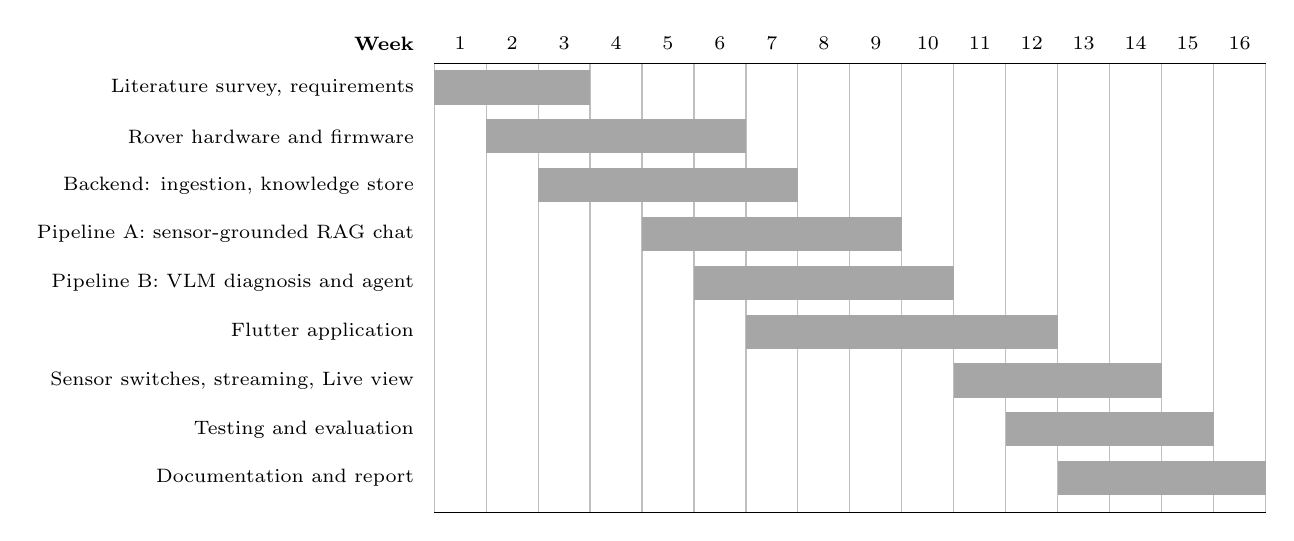
\begin{tikzpicture}[x=0.66cm,y=-0.62cm]
\def\bar#1#2#3#4{\fill[black!35] (#2-1,#1+0.15) rectangle (#3,#1+0.85);\node[anchor=east,font=\scriptsize] at (-0.2,#1+0.5) {#4};}
\foreach \w in {1,...,16} {\node[font=\scriptsize] at (\w-0.5,-0.4) {\w};\draw[black!25] (\w-1,0) -- (\w-1,9.2);}
\draw[black!25] (16,0) -- (16,9.2);
\node[font=\scriptsize\bfseries,anchor=east] at (-0.2,-0.4) {Week};
\draw (0,0) -- (16,0);
\bar{0}{1}{3}{Literature survey, requirements}
\bar{1}{2}{6}{Rover hardware and firmware}
\bar{2}{3}{7}{Backend: ingestion, knowledge store}
\bar{3}{5}{9}{Pipeline A: sensor-grounded RAG chat}
\bar{4}{6}{10}{Pipeline B: VLM diagnosis and agent}
\bar{5}{7}{12}{Flutter application}
\bar{6}{11}{14}{Sensor switches, streaming, Live view}
\bar{7}{12}{15}{Testing and evaluation}
\bar{8}{13}{16}{Documentation and report}
\draw (0,9.2) -- (16,9.2);
\end{tikzpicture}}

\caption{Project timeline (weeks).}
\label{fig:gantt}
\end{figure}
